\chapter{Vorlesung 11}
\section{AVL-Bäume von Adelson-Velskii and Landis}

\begin{figure}
    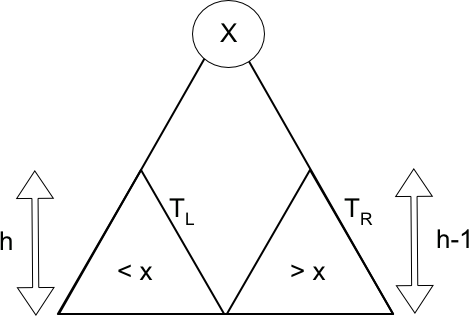
\includegraphics[width=0.6\textwidth,left]{Grafik/img1.png}
    \caption{left aligned image}
\end{figure}


\paragraph{Ziel:}%%2 Bilder einfügen
Zeige, dass die maximale Tiefe eines AVL-Baums mit n Knoten ($\hat{=}~ n$ gespeicherten Schlüsseln) $O(\log(n))$ beträgt.\\
$\Rightarrow$ Suchzeit $O(\log(n))$ im worst case.


